\section{System Design}
\label{sec:design}

\begin{figure*}[t]
  \centering
  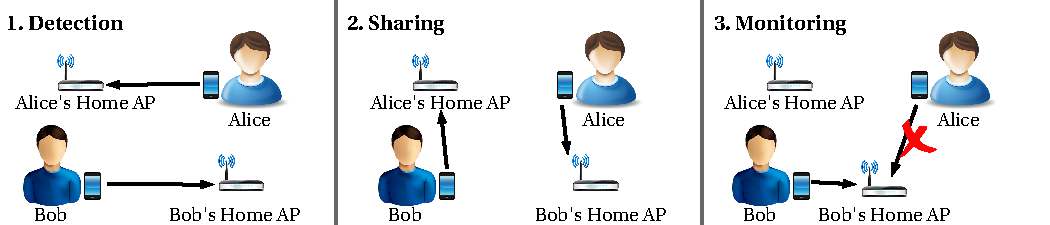
\includegraphics[width=\textwidth]{./figures/design.pdf}
  \caption{\textbf{\wisefi{} System Work Flow.}}
  \label{fig:design}
\end{figure*}

Inspired by the results of the investigation in Section~\ref{sec:investigation},
we design a system called \wisefi{} to detect reciprocal sharing
opportunities (\S\ref{subsec:detection}), enable \wifi{} sharing
(\S\ref{subsec:sharing}) and monitor the \wifi{} performance to ensure the
sharing remains reciprocal (\S\ref{subsec:monitoring}). Figure~\ref{fig:design}
shows the overall work flow of the \wisefi{} system.

\subsection{Detection}
\label{subsec:detection}

To detect reciprocal sharing opportunities, two information are required: the
home AP of the device, and neighbor APs' signal strength during \wifi{} sessions
with the home AP. A smartphone application can be deployed through app market
to collect these information. In particular, the home AP information can be
learned over a period of time using the heuristics developed in
Section~\ref{subsec:homeap}, or be inputed directly by user. \wifi{} scan
results during sessions with home APs can then be logged to identify the
neighbor APs that can potentially provide better signal. Finally, these
information are uploaded and fused in \wisefi{} server to identify reciprocal
sharing opportunities using the methods described in Section~\ref{subsec:reciprocal}.

\subsection{Sharing}
\label{subsec:sharing}

Once the reciprocal sharing opportunities are discovered, the \wisefi{} server
can distribute such information to the \wisefi{} application on smartphone,
which will prompt users to establish \wifi{} sharing. The sharing mechanism must
meet two goals: control and protection. First, the system should be able to
control the sharing, including granting the access of home AP to other \wisefi{}
users, and revoking the access when the reciprocal sharing opportunity no longer
exists.  Second, the system should protect the home network from other \wisefi{}
users by sharing access only to the Internet, and protecting private resources
such as home network printers or storage.

Some mid-to-high end wireless routers support the \textit{virtual network}
feature, where multiple virtual \wifi{} networks are emulated by a single router
hardware, and different network parameters, such as SSID, bandwidth cap, access
permission, can be enforced separately for each virtual network. This feature is
typically used to set up a guest \wifi{} network to provide network access to
temporal visitors yet isolate them from home clients. For home APs with such
feature, \wifi{} sharing can be achieved by only distributing the credential of
guest network to other \wisefi{} users. Access and bandwidth policies can then
be enforced on the guest network to achieve control and protection.
Additionally, such isolation and enforcements are mostly likely already enabled
by default for guest networks, so that even inexperienced user can configure the
\wifi{} sharing through guest network.

For APs without guest network feature, however, cumbersome AP configurations may
be required by user, such as MAC black or white list, routing table
modification, etc.  Such configurations are probably too complicated for average
users to perform.  We discuss this challenge and possible solutions in
Section~\ref{subsec:config}.


\subsection{Monitoring}
\label{subsec:monitoring}

After the sharing is established, the system needs to monitor both \wifi{}
\textit{usage} and \textit{performance} of both parties to ensure that the
sharing remains reciprocal.  There are two reasons why this is necessary: one is
obvious and another is obscure.

First, it is obviously important to ensure that the sharing remains reciprocal
in long term to provide incentives for both parties to participate the sharing.
For instance, suppose the system has established reciprocal \wifi{} sharing
between Alice and Bob, and Bob decides to deploy an extra AP at his home which
makes him no longer benefit from sharing Alice's home AP. The system should
monitor Bob's \wifi{} usage to detect the termination of the reciprocal
relationship and revoke Alice's access of Bob's home AP accordingly.

Second, the not so obvious reason is that, as mentioned in
Section~\ref{subsec:better}, \wifi{} signal strength is used as a hint to
identify potentially better APs. And it is well known that signal strength does
not directly translate to \wifi{} performance. Other factors, such as AP load,
modulation, interference, or \wifi{} generation, also affect the link quality
yet can not be easily detected by the smartphone. Furthermore, last hop \wifi{}
link quality does not necessarily determines clients' overall end-to-end network
performance. In fact, there is no way to determine whether the neighbor AP can
indeed provide better network performance than user's home AP until the sharing is
actually established.

To measure the reciprocity in terms of network performance, standard performance
benchmarks, such as download/upload throughput, \texttt{ping} latency, or DNS
lookup, can be performed periodically by the \wisefi{} client. However, it is
not trivial to monitor the network usage side of reciprocity from the vantage
point of a single client: the smartphone's association time may not be
representative of user's other wireless devices. We return to this matter in
Section~\ref{subsec:config} to discuss possible solutions.
